\chapter{Coding style}
\newpage

Coding style là gì? Nếu như bạn thấy code của bạn rối tung rối mù, lấy code của thằng bạn đọc để fix bug cho nó mà đọc muốn rớt con mắt ra ngoài, hay thêm một tính năng mới rồi okie, bỏ hết cái mớ code rồi ngồi code lại.

Và coding style giúp bạn giải quyết mấy chuyện đó, tuyệt vời!!! Và làm sao mà nó có thể làm được vậy?

Có 3 yêu cầu chính mà người lập trình cần đáp ứng cho chương trình: chạy được, dễ thay đổi, dễ hiểu.
\begin{itemize}
  \item Chạy được: Tất nhiên là mọi người đều hướng tới mục tiêu này, không chạy được thì có code cũng như không.
  \item Dễ thay đổi: yếu tố chạy được là đáp ứng được tiêu chí đề ra. Nhưng mà với lập trình thực tế thì các tiêu chí đó liêu tục bị thay đổi. Giống như việc ông sếp thấy phương án này chua ăn quá nên đổi qua cái kia, ông khách hàng thì muốn thêm tính năng này, đề xuất cái kia. Ví dụ như bạn đi, làm một cái xe nhỏ nhỏ dò line, làm xong rồi muốn gắn cái camera vô xử lý ảnh cho chạy, làm xong rồi nữa thì muốn gắn thêm đèn chớp chớp cho vui chẳng hạn. Hoặc mục tiêu bạn đâu thực hiện xong rồi mà thấy nó chạy chưa ngon, muốn viết lại xíu để nâng cấp firmware lên, giờ nhìn vô cái đống bùng nhùng kia hông lẽ đập đi xây lại?
	\item Dễ hiểu: vì các dự án thực tế đều cần làm nhóm cả. Bạn sử dụng code của người khác để viết thêm, người sau này sẽ dùng code của bạn thể phát triển, nâng cấp bảo trì chẳng hạn. Hoặc chính bạn sau một thời gian đọc lại code của mình có khi không biết ngày xưa mình vẽ bùa gì trong đây nữa. Nên code phải viết làm sao cho người khác có thể đọc được (tất nhiên thằng đó nó phải được được xíu, đừng có gà quá).
\end{itemize}

Và coding style là cái cách bạn viết chương trình để đáp ứng các yêu cầu trên.

Có thể khẳng định thế này, lập trình không có khó, ngồi fix bug mới mệt. Thế nên việc có coding style sẽ làm cho cuộc sống của bạn dễ chịu hơn rất nhiều. Ngoài việc chịu khó ngồi code là còn phải đọc sách hoặc thỉnh giáo cách sư phụ để làm thế nào cho công việc nó hiệu quả hơn.

Rồi đến một ngày bạn sẽ thấy ngồi viết code cũng giống như viết văn xuôi vậy.
\newpage
\section{Moudule hóa}

Mọi hệ thống lớn đều hợp thành từ những thành phần nhỏ, hãy chia nhỏ chương trình ra thành các module, file có chức năng khác nhau để dễ quản lý.
\begin{figure}[h!]
\centering
 \includegraphics[width=0.6\linewidth]{images/module.png}
 \caption{Module hóa trong KeilC}
\end{figure}

Trong keilC, các file có chức năng tương đương nhau được gộp vào các thư mục.

Còn trong Arduino thì hơi củ chuối hơn xíu, bạn phải bỏ toàn bộ file vô cùng thư mục với file .ino. Nếu có rất nhiều file thì nhìn sẽ rối.
\newpage 
\begin{figure}[h!]
\centering
 \includegraphics[width=1\linewidth]{images/arduino_folder.png}
 \caption{Thư mục Arduino}
\end{figure}

Nhưng cũng tạm ổn. Và đây là thành quả
\begin{figure}[h!]
\centering
 \includegraphics[width=0.8\linewidth]{images/arduino.png}
 \caption{Module hóa trong Arduino}
\end{figure}

Mình từng gặp mấy bạn mới code viết tất cả mọi thứ vào hàm main (kinh dị) từ đọc cảm biến, đọc nút nhấn, điều khiển động cơ... Bạn nên viết hoặc sử dụng thư viện cho mỗi loại phần cứng đó, rồi trong hàm main chỉ gọi hàm trong thư viện đó ra.

Nguyên tắc để chia module: module A có thể biết module B làm được \textbf{cái gì} nhưng nó không biết module B làm điều đó \textbf{như thế nào}. Ví dụ bạn sử dụng hàm \textit{Serial.write()} trong Arduino chẳng hạn, bạn biết chắc chắn nó sẽ chuyển dữ liệu đi cho bạn nhưng bạn không cần biết nó chuyển đi như thế nào. A giao việc cho B theo phương thức quy định sẵn và chấm hết. B có thể báo về cho A một số trạng thái như công việc có thành công hay không, hoặc thất bại do nguyên nhân gì.

Yêu cầu như trên làm tăng tính độc lập cho các module với nhau, làm cho cả chương trình trở nên rõ ràng hơn. Ví dụ khi lỗi xảy ra, bạn có thể biết được ở A hay B gây ra lỗi, khoanh vùng lỗi nhỏ hơn để dễ kiếm hơn. Khi bạn muốn nâng cấp B để nó chạy nhanh hơn, những chương trình ở A viết sử dụng hàm mà B cung cấp sẽ vẫn hoạt động bình thường, không phải sửa lại mọi thứ. Các thư viện trong Arduino vẫn thường xuyên được cập nhật nhưng chương trình bạn viết vẫn chạy được là vì lí do này.

\section{Cấu trúc chương trình chính và cách gọi hàm}

Hàm main trong chương trình chính thường có cấu trúc là khởi tạo và vòng lặp chương trình. 
\begin{lstlisting}
void main(void)
{
	system_init();
	
	while(1)
	{
		//Do what you want
	}
}
\end{lstlisting}

Tương tự như arduino nó có setup() và loop().
\begin{lstlisting}
void setup() {
  // put your setup code here, to run once:

}

void loop() {
  // put your main code here, to run repeatedly:

}
\end{lstlisting}

Ví dụ như mình viết một chương trình đọc cảm biến và 10 phút gửi về một lần. Thì mình sẽ viết như sau:
\begin{lstlisting}
void main(void)
{
	system_init();
	
	while(1)
	{
		read_sensor();
		send_data();
		delay(10_minutes);
	}
}
\end{lstlisting}

Bạn thấy không, chương trình mình viết nó y chang những gì mình nói. Còn việc các hàm đọc cảm biến read\_sensor() hoặc gửi dữ liệu về send\_data() nó ra sao trong đó thì viết ở chỗ khác. Đừng nhét mọi thứ mà bạn có thể viết ra vào đây, làm ơn!!!

Có một khái niệm về \textbf{mức trừu tượng}. Ví dụ như hàm đọc cảm biến read\_sensor có thể bao gồm 3 hàm thế này:
\begin{lstlisting}
void read_sensor(void)
{
	request_sensor_data();
	wait_for_sensor_data();
	save_sensor_data();
}
\end{lstlisting}
đầu tiên ra lệnh cho cảm biến, sau đó chờ và khi dữ liệu về thì cất đâu đó. Bạn có thể thấy mức trừu tượng của hàm read\_sensor sẽ cao hơn 3 hàm trong đó vì nó bao hàm 3 cái hàm này. Hàm read\_sensor thì có mức trừu tượng bằng với hàm 2 hàm còn lại trong vòng while(1) của hàm main vì đây là 3 bước tuần tự nhau trong một công việc.

Nói tóm lại hãy phân thứ bậc cho các hàm (như mô hình đa cấp ấy :) và khi một hàm gọi các hàm con thì nhớ rằng các hàm con nên có cùng mức trừu tượng với nhau.
\begin{figure}[h!]
	\centering
	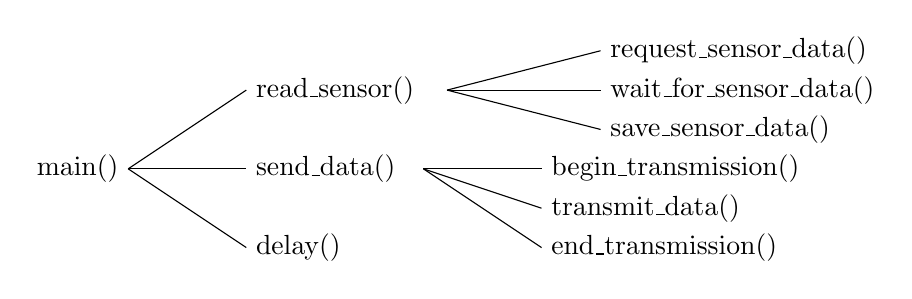
\begin{tikzpicture}[yscale=0.5, xscale=1.5]
	\node [left] at (0, 0) {main()};

	\draw (0,0) -- (1, 2);
	\node [right] at (1,2) {read\_sensor()};
		\draw (2.7,2) -- (4, 3);
		\node [right] at (4,3) {request\_sensor\_data()};
		\draw (2.7,2) -- (4, 2);
		\node [right] at (4,2) {wait\_for\_sensor\_data()};
		\draw (2.7,2) -- (4, 1);
		\node [right] at (4,1) {save\_sensor\_data()};
	\draw (0,0) -- (1, 0);
	\node [right] at (1,0) {send\_data()};
		\draw (2.5,0) -- (3.5, 0);
		\node [right] at (3.5,0) {begin\_transmission()};
		\draw (2.5,0) -- (3.5,-1);
		\node [right] at (3.5, -1) {transmit\_data()};
		\draw (2.5,0) -- (3.5, -2);
		\node [right] at (3.5, -2) {end\_transmission()};

	\draw (0,0) -- (1, -2);
	\node [right] at (1,-2) {delay()};
	
		
	\end{tikzpicture}
	\caption{Mô hình đa cấp.}
\end{figure}

Nhớ là hông phải mình làm màu mà viết tên hàm tiếng Anh đâu, vì tiếng Việt không dấu nó như teencode vậy đọc không nổi, mà nhiều khi hiểu lộn nghĩa :).
\section{Hàm số}

Việc phát minh ra các hàm con là phát minh vĩ đại như phát minh ra cái máy tính vậy. Nếu không có hàm con thì bạn tưởng tượng viết chương trình một lèo từ đầu tới cuối xem.

Vậy nên để đạt hiệu quả thì cần có những lưu ý sau:
\subsection{Đặt tên hàm}

Tên hàm được đặt để cho biết cái \textbf{hàm con đó nó làm cái gì}. Ví dụ như read\_sensor() chẳng hạn, dù bạn chưa biết cảm biến loại gì và đọc nó như thế nào nhưng cũng hiểu sơ sơ về mục đích gọi hàm.

Và hàm \textbf{nên chỉ thực hiện một chức năng duy nhất}. Nó chỉ làm những gì mà tên hàm nói đến, không hơn không kém. Trong khi viết code thì mọi thứ nên được viết tường minh ra. Ví dụ như hàm gọi hàm send\_data() để truyền dữ liệu về, nếu khi truyền xong muốn xóa dữ liệu cũ đi thì gọi hàm delete\_data() sau khi gọi hàm send\_data().
\begin{lstlisting}
while(1)
{
	read_sensor();
	send_data();
	delete_data();
	delay(10_minutes);
}
\end{lstlisting}
Không nên nhét hàm delete\_data() vào bên trong send\_data() như muốn hiểu ngầm "gửi xong rồi xóa nó đi chứ để làm gì". Vì nhiều khi có việc cần đến nó. Việc viết tường mình, tránh những chỗ hiểu ngầm sẽ giúp người đọc nắm đủ các bước thực hiện của bạn. 

Hàm được thực thi càng chính xác với cái tên của nó bao nhiêu thì code của bạn sẽ càng dễ đọc bấy nhiêu. 

Một vài ví dụ như khi viết vội có bạn đặt tên hàm kiểu ham\_a(), ham\_b(), hoặc func\_1(), func\_2(), mai mốt đọc lại xỉu.

Việc bạn đặt tên hàm rồi sau thấy củ chuối quá thì cũng đừng ngại đổi lại, mình nhiều khi cũng phải đổi 2-3 lần mới được cái tên vừa ý.

Hãy viết theo kiểu cho một người chưa biết gì về chương trình của bạn đọc. Và đặc biệt tránh kiểu viết trẻ trâu thích thể hiện, viết đoạn code thật ngầu, thật nhỏ xíu mà vẫn chạy ngon. Sau này chỉ khổ cho mấy người phải đọc lại nó.
\subsection{Độ dài của hàm}

Nguyên tắc để dễ code dễ đọc: code ngắn thôi, với lại tên hàm đặt đúng với yêu cầu. 

Một số hàm chỉ hoạt động tốt nếu nó đủ dài, cắt ngắn lại thành ra dở. Tuy nhiên đa số các trường hợp bạn có thể cắt một hàm dài bất tận ra thành các hàm nhỏ, như chia giai đoạn ra, rồi đặt tên hàm theo các giai đoạn của chương trình. Rất thường xuyên hàm viết ra để gọi có một lần, nó không có tác dụng là tránh lặp lại code như mục đích sinh ra hàm ban đầu, nó chỉ có tác dụng làm chương trình bạn gọn gàng hơn, dễ đọc hơn.

Còn độ dài của nó bao nhiêu là vừa. Cái này bạn phải làm rồi rút ra kinh nghiệm cho bản thân. Với mình thì dài dưới 10 dòng là okie nhất, trên 20 dòng thì nên cắt nó đi.
\subsection{Truyền tham số}

Tham số là nơi giao tiếp của hàm này với hàm kia. Nó là nơi giao thương nên giống như cái chợ vậy, rất nhiều vấn đề phát sinh. Mà nói chung là một hàm nên hạn chế các tham số đầu vào, chỉ giữ lại nhưng tham số tối quan trọng. Bạn viết một hàm với yêu cầu truyền 5 cái thông số đầu vào thì làm sao bạn nhớ được thứ tự của tham số đó mà truyền cho đúng?
%viet tiep
\subsection{Bảo vệ hàm số}

Giả sử bạn viết một hàm chia a cho b như sau:
\begin{lstlisting}
float a_divide_b(int a, int b)
{
	return (float)a/b;
}
\end{lstlisting}


Rồi bỗng một ngày đẹp trời, một thanh niên lấy hàm bạn viết ra, rồi xài như sau: \textit{float result = a\_divide\_b(2, 0)}. Xong biên dịch thì không báo lỗi nhưng mà chạy cái nó xịt khói. Đây là lỗi chia cho 0, thành ra nó không tính được và chạy loạn xạ.

Thế nên với mỗi chương trình có truyền tham số vào, hãy nhớ là kiểm tra coi nó có hợp lệ hay không, nếu tính toán thì tham số đưa vào có thuộc tập xác định hay không... Bởi vì bạn sẽ không biết sau này người nào đó (ngay cả bạn nữa) dùng hàm sẽ truyền cái gì vào trong đó nên phải kiểm tra lại. Nguyên tắc kiểm tra là : không tin cha con thằng nào cả. Đừng hi vọng ai đó sẽ truyền vào tham số hợp lệ, thường thì họ chả quan tâm đâu. Nên nhớ kiểm tra đầu vào hợp lệ thì mới thực thi hàm.

Hàm có kiểm tra tham số đầu vào:
\begin{lstlisting}
float a_divide_b(int a, int b)
{
	if(b==0){
		//printf("Divided by 0 error\n");
		return 0;
	}
	return (float)a/b;
}
\end{lstlisting}

\section{Các biến số}

Tất nhiên là khi lập trình bạn đều phải khai báo biến, rồi sử dụng các biến đó để lưu trữ, tính toán. Thế nên việc sử dụng cẩn thận các biến là điều rất quan trọng để chương trình có thể chạy được và ít phát sinh lỗi.
\subsection{Đặt tên biến}

Cũng giống như việc đặt tên hàm, một biến được đặt tên để biến nó sinh ra để làm cái gì. Bạn có thể thấy cách mà mình đặt tên cho kiểu \textit{env\_t}, bao gồm \textit{temp, humi, lux}, nếu bạn sử dụng quen thì có thể biết từng biến trong đó lưu giá trị gì mà không bị nhầm lẫn (viết tắt của temperature, humidity, lux). Có nhiều bạn sử dụng các chữ cái như a, b, c... hoặc x1, x2 để đặt tên biến, nhưng mà tin mình đi, mấy cái đó đọc nhức mắt kinh khủng, đôi khi trong lúc code bạn cũng không nhớ khai báo nó để lưu cái gì nữa. Tại hại hơn là bạn lại lưu vào x1 giá trị đáng lí ra phải lưu vào x2.

Theo thói quen thì cái chữ cái như i, j... được dùng trong vòng lặp cho tiện. Điều này cũng không có vấn đề gì nhiều nếu bạn sử dụng quen nó. Nhưng còn cái loại biến khác thì hãy đặt cho nó cái tên gắn liền với chức năng của nó.

Một ví dụ về tìm số lớn nhất trong một mảng như sau:
\begin{lstlisting}

uint8_t array[100];
void main(void){
	//enter the array
	uint8_t arr_max=0;
	for(uint8_t i=0; i<100; i++){
		if(arr_max < array[i]){
			arr_max=array[i];
		}
	}
	printf("Maximum value of array: %d\n", arr_max);
}

\end{lstlisting}


Đó là ví dụ về cách đặt tên viết với arr\_max chỉ giá trị lớn nhất của mảng (array's maximum value). Nhưng có một vấn đề là trong vòng lặp for, số 100 đó có nghĩa là gì? Chắc là số lượng của mảng. Chúng ta có thể biết vì đây là chương trình đơn giản. Nhưng còn nếu chương trình với những thuật toán phức tạp, vài cái vòng lặp chồng lên nhau, với lại chương trình mấy trăm dòng thì câu chuyện sẽ khác. Mình chắc là sẽ phải tìm một hồi mới ra coi số 100 đó là gì.

Thế nên trong code cũng không nên xuất hiện con số nào cả. Hãy đặt cho mỗi con số một cái tên.

\begin{lstlisting}
#define ARRAY_SIZE 100
uint8_t array[ARRAY_SIZE];
void main(void){
	//enter the array
	uint8_t arr_max=0;
	for(uint8_t i=0; i<ARRAY_SIZE; i++){
		if(arr_max < array[i]){
			arr_max=array[i];
		}
	}
	printf("Maximum value of array: %d\n", arr_max);
}

\end{lstlisting}

Các bạn có thể thấy là việc đọc nó giờ sẽ trở nên đơn giản hơn rất nhiều. Với lại mỗi lần muốn sửa lại kích thước mảng thì mình chỉ cần sửa một chỗ thôi.
\subsection{Các lưu ý khi khai báo biến}

Khi khai báo và sử dụng biến nên chú ý những điểm sau:
\begin{itemize}
\item Tránh sử dụng biến toàn cục (global variable): biến toàn cục được khai báo bên ngoài hàm, là nơi mà bất kì hàm nào cũng có thể truy cập và chỉnh sửa nó. 
\begin{lstlisting}
int a; //this is a global variable

void setup(){
}

void loop(){
}
\end{lstlisting}

Hãy tưởng tượng là trong file này của bạn có khoảng 20 hàm được khai báo, mà hàm nào cũng có quyền truy cập vào biến toàn cục này, nên bất cứ lúc nào nó cũng có thể bị thay đổi. Tệ hơn nữa nếu không phải do một mình bạn viết mà do vài người viết nên file code này, việc không hiểu rõ ý mà tự tiện truy cập vào biến toàn cục là chuyện bình thường.

Thế nên hãy hạn chế biến toàn cục hết mức có thể, và tốt nhất là không khai báo biến kiểu này càng tốt. Khi nhất thiết phải sử dụng biến toàn cục thì nên chú thích rõ những nơi nào được đọc, ghi biến này để tránh việc thay đổi biến mà không biết trước.

Biến toàn cục là đồ công cộng. Ai cũng đụng chạm nó được. Mà đồ công cộng thì không an toàn. Thế thôi.
\item Hãy khởi tạo giá trị cho biến: Thay vì khai báo \textit{int a;} thì hãy khai báo \textit{int a=0;}. Đôi khi việc bạn khai báo biến thì CPU chỉ định vị biến này trong bộ nhớ mà không tự khởi tạo biến này với giá trị mặc định là 0 có thể gây lỗi, nhất là ngay sau đó bạn dùng phép toán \textit{or} chẳng hạn.
\item Luôn chắc rằng biến của bạn có thể chứa đủ giá trị mà bạn muốn lưu vào trong đó. Ví dụ như việc sử dụng biến uint8\_t, với khoảng giá trị từ 0 tới 255, nếu tình cờ mà bạn ghi vào con số lớn hơn khoảng giá trị này thì nó sẽ xịt khói lập tức.
\end{itemize}
\subsection{Kiểu biến static}

Kiểu biến \textit{static} hay thường gọi là biến tĩnh. Nó được khởi tạo một lần và chạy suốt với chương trình đến khi chương trình kết thúc.

Có một ví dụ sau trong DevC++:
\begin{lstlisting}

void print_example(){
	int a=0;
	a++;
	printf("a= %d\n", a);
	
	static int b=0;
	b++;
	printf("b= %d\n", b);
}

void main(void){
	print_example();
	print_example();
}

\end{lstlisting}

Ở lần gọi hàm print\_exmaple đầu tiên, nó sẽ in ra a=1, b=1, nhưng đến lần thứ 2, nó sẽ in ra a=1, b=2. 

Nếu như biến thường không có khai báo \textit{static}, nếu là biến được khai báo trong hàm thì khi kết thúc hàm biến đó sẽ bị mất đi, và khi gọi hàm lại thì nó sẽ được khai báo lại. Còn đối với kiểu biến
\textit{static}, nó sẽ vẫn tồn tại khi kết thúc gọi hàm, và khi gọi hàm lần nữa, nó sẽ bắt đầu với kết quả từ lần gọi hàm lần trước. Hay nó cách khác, biến \textit{static} có thời gian sống như biến toàn cục nhưng phạm vi truy cập chỉ trong một hàm thôi. 

Việc mình đề cập tới nó ở đây vì sử dụng biến kiểu \textit{static} để hạn chế các biến toàn cục đi, quây biến lại trong một hàm nào đó thôi, và dùng khi nào cần lưu kết quả lại cho lần gọi hàm sau.
\subsection{Kiểu biến volatile}

Biến volatile được khai báo khi biến đó có thể thay đổi giá trị không báo trước. Việc báo trước có nghĩa là bạn sẽ có lệnh gán như a=0 hoặc b=1 tường minh ở trong chương trình. Còn sau đây là các trường hợp biến thay đổi mà không báo trước như sau:
\begin{itemize}
\item Thanh ghi ngoại vi có ánh xạ đến ô nhớ (Memory-mapped peripheral registers), bạn có thể hiểu nôm na là biến đó lưu trữ trạng thái hiện tại của một chân I/O nào đó, nó có thể thay đổi do tác động bên ngoài.
\item Biến toàn cục được truy xuất từ các tiến trình con xử lý ngắt: Chương trình của bạn có thể chia làm 2 phần, một phần là chương trình chính và một phần phục vụ ngắt. Khi có ngắt xảy ra, nó sẽ tạm dừng chương trình chính để thực hiện tác vụ ngắt tương ứng. Tác vụ ngắt này có thể thay đổi một biến toàn cục như là một cái cờ (flag) để chương trình chính biết là có ngắt xảy ra.
\item Biến toàn cục được truy xuất từ nhiều tác vụ trong một ứng dụng đa luồng: người ta có thể tận dụng sức mạnh của MCU bằng viết chương trình đa luồng bằng cách sử dụng hệ điều hành như FREERTOS chẳng hạn, đại khái là viết 2 chương trình chính chạy đồng thời với nhau. Thì một biến toàn cục có thể được chương trình này thay đổi nhưng chương trình kia không biết khi nào.
\end{itemize}

Bạn có thể xem thêm ở đây: \url{http://ktmt.github.io/blog/2013/05/09/y-nghia-cua-tu-khoa-volatile-trong-c/}
\section{Chú thích}

Chú thích (comment) tưởng đơn giản nhưng lại là thành phần hại não trong khi viết chương trình. Bạn có thể thấy trong C thì chú thích đi sau dấu // hoặc /* */. Tại sao nó hại não? Vì nếu chú thích đúng cách thì chương trình rất dễ đọc và người khác (ngay cả bạn nữa) cũng nắm được đại ý nhanh chóng. Nhưng khổ cái là chương trình thay đổi liên tục, mà hễ thay đổi thì chỉnh sửa code lại thôi, không ai chịu sửa lại chú thích làm chi (vì sửa code không cũng đuối rồi). Nên làm cho người đọc tưởng là mình hiểu rồi nhưng một hồi đọc tới code thì thấy nó sai sai.

Thế nên cách chú thích tốt nhất là hạn chế nó hết mức có thể. Sử dụng tên hàm, tên biến như là một loại chú thích hiệu quả hơn.

Tất nhiên là bạn không nên bỏ hẳn nó đi, vì nếu sử dụng nó đúng cách thì nó đem lại hiệu quả rất nhiều. Các chương trình thường đặt chú thích lên đầu trang để giải thích khái quát coi chương trình đó đùng để làm gì. Trong file \textit{.h}, các chú thích được đặt trước tên hàm giải thích công dụng của hàm đó, để người sử dụng có thể sử dụng luôn thư viện mà không cần phải đọc tới file code. Đôi khi những đoạn code khó đọc, tính logic cao thì nên có chú thích để giải thích coi ý tưởng đằng sau đoạn code đó là gì, nó giải quyết vấn đề gì.

\section{Lưu đồ giải thuật}

Có bạn nào viết lưu đồ giải thuật (flowchart) ra rồi mới code không, hay toàn làm ngược lại, code rồi mới viết lưu đồ ra cho có rồi đem nộp?

Lưu đồ giải thuật thường viết khi bạn thực hiện một đoạn chương trình khó, nặng tính logic. Còn thông thường thì không cần nó làm chi. Hồi sinh viên viết mấy đoạn dễ ẹc nên không bao giờ mình viết lưu đồ ra, có viết thì để làm báo cáo thôi. Giờ đi làm gặp những thứ chua ăn hơn, nếu không viết nó ra thì không biết code thế nào cho đúng. 

Và lưu đồ giải thuật sẽ tập cho bạn thói quen suy nghĩ trước khi làm, chứ không phải là làm theo cảm tính rồi ngồi sửa. Hãy nhớ code chỉ là một phần của sản phẩm bạn tạo ra, hãy dành thời gian suy nghĩ về cấu trúc của sản phẩm, thiết kế từng module rồi vẽ lưu đồ nếu cần. Đó là bước bạn làm cho ý tưởng của bạn nó rõ ràng, cách diễn đạt được mạch lạc. Cuối cùng là chỉ cho cái máy hiểu bạn muốn nó làm cái chi (là viết chương trình đó). Đừng cắm đầu code khi bạn còn chưa biết bạn sẽ làm cái gì nữa.

Rồi một ví dụ về bên nhận dữ liệu uart (lại là uart). Bên nhận thì nhìn chung không biết thằng phát sẽ phát bao nhiêu, nó không biết bao giờ sẽ kết thúc cái chuỗi mà nó đang nhận. Vậy làm thế nào để khi bên phát hết phát thì bên thu sẽ biết mà còn đi làm cái khác?

Có rất nhiều cách. Như người ta có thể chuyển dữ liệu sang chỗi json (đại khái toàn là chuỗi kí tự mã ASCII và dữ liệu không bao giờ có kí tự kết thúc chuỗi '\textbackslash0') và sau đó thêm kí tự '\textbackslash0' vào cuối chuỗi, bên nhận nhận được kí tự này và báo về chương trình chính đã nhận xong. Nhưng ở đây mình sử dụng cách đơn giản hơn, nếu nó đang nhận dữ liệu và đột nhiên không nhận được nữa trong vòng 20 mili giây thì nó sẽ báo là nhận xong rồi.

Rồi viết ra yêu cầu của chương trình rồi giờ tới thiết kế. Bạn tự làm thử xem :)))

Theo yêu cầu thì bộ truyền nhận sẽ có 2 trạng thái: WAITING (đang chờ dữ liệu, kí hiệu WAIT=0) và RECEIVING (đang nhận, kí hiệu RECV=1). Khi mới khởi tạo thì nó sẽ có trạng thái đang chờ. Khi nhận được thông báo có dữ liệu đến thì nó sẽ chuyển qua trạng thái đang nhận. Nhận xong thì trở về WAITING.
\begin{figure}[h!]
	\centering
\begin{tikzpicture}[->,>=stealth',shorten >=1pt,auto,node distance=5cm,
                    semithick]

  \node[initial,state] (A)                    	{$WAIT$};
  \node[state]         (B) [right of=A] 		{$RECV$};

  \path (A) edge [bend left]            node {data} (B)
        (B) edge [loop above] 			node {data} (B)
            edge [bend left]            node {timeout} (A);
 
\end{tikzpicture}
\caption{Lưu đồ máy trạng thái.}

\end{figure}

Trên là lưu đồ đơn giản nhất. Trong chương trình mình sẽ viết theo kiểu non-blocking, tức là không có sử dụng hàm delay() mà chương trình sẽ liên tục kiểm tra ngõ vào. Tài nguyên có hạn nên bạn không nên phung phí nó mà sử dụng hàm delay(), chương trình sẽ đứng nguyên một chỗ. Có thời gian thì mình sẽ viết chi tiết hơn.

Rồi giờ tới lưu đồ cho anh kia.
\begin{figure}
\centering
\begin{tikzpicture}[node distance=2cm]

\node (start) [startstop] {Begin};
\node (dec1) [decision, below of=start, yshift=-0.5cm] {state=0?};
\draw [arrow] (start) -- (dec1);

\node (dec2) [decision, left of=dec1, xshift=-1cm] {data?};
\draw [arrow] (dec1) -- node [above] {Y} (dec2);

\node (dec3) [decision, right of=dec1, xshift=1cm] {data?};
\draw [arrow] (dec1) -- node [above] {N} (dec3);

\node (pro1) [process, right of=dec3, xshift=1cm] {get data?};
\draw [arrow] (dec3) -- node [above] {Y} (pro1);
\node (dec4) [decision, below of=dec3, yshift=-0.5cm] {timeout?};
\draw [arrow] (dec3) -- node [right] {N} (dec4);


\node (stop) [startstop, below of=start, yshift=-10cm ] {End};
\draw [arrow] (pro1) |-  (stop);
%\node (pro2a) [process, below of=dec1, yshift=-0.5cm] {Process 2a};
%\node (stop) [startstop, below of=out1] {Stop};
%\draw [arrow] (start) -- node [right] (dec1);

\end{tikzpicture}
\caption{Lưu đồ giải thuật.}
\end{figure}


\end{comment}